\documentclass[conference]{IEEEtran}

\usepackage[T1]{fontenc}
\usepackage[utf8]{inputenc}
\usepackage{amsmath,amssymb}
\usepackage{graphicx}
\usepackage{subcaption}
\usepackage{booktabs}
\usepackage{siunitx}
\usepackage{url}
\usepackage[hidelinks]{hyperref}

\sisetup{separate-uncertainty=true,detect-all=true}
\graphicspath{{../figuras/}{../figuras/fotos/}}

% Numerical values written by scripts/run_all.py
% Archivo generado por scripts/run_all.py -- no editar a mano
\newcommand{\NFrames}{20}
\newcommand{\PixelUm}{4.65}
\newcommand{\DetWidthMm}{5.95}
\newcommand{\HartLamZero}{246.93}
\newcommand{\HartC}{$-$162304}
\newcommand{\HartXzero}{1396.9}
\newcommand{\CalRMS}{0.35}
\newcommand{\CalN}{7}
\newcommand{\NFeatures}{14}
\newcommand{\CurvSagitta}{42}
\newcommand{\CurvRMS}{0.92}
\newcommand{\CurvTilt}{$-$2.2}
\newcommand{\RangeMin}{424}
\newcommand{\RangeMax}{726}
\newcommand{\RangeThr}{5}
\newcommand{\RangeDetMin}{363}
\newcommand{\RangeLastLine}{966}
\newcommand{\RangeThMin}{416}
\newcommand{\RangeThMax}{1000}
\newcommand{\FlashSat}{6.5}
\newcommand{\DispMeasFiveH}{0.39}
\newcommand{\DispMeasSixH}{0.77}
\newcommand{\DispMeasEightH}{1.88}
\newcommand{\DispThFiveH}{0.26}
\newcommand{\DispThSixH}{0.52}
\newcommand{\DispRatio}{1.47}
\newcommand{\DispRatioSpread}{3}
\newcommand{\FCamEff}{27.3}
\newcommand{\RMin}{58}
\newcommand{\RMax}{301}
\newcommand{\RThFFS}{197}
\newcommand{\RThEES}{77}
\newcommand{\RDiffFiveH}{3241}
\newcommand{\SlitImgUm}{33.3}
\newcommand{\SlitImgPx}{7.2}
\newcommand{\FWHMKr}{3.2}
\newcommand{\FWHMAr}{3.7}
\newcommand{\ThetaInc}{59.7}
\newcommand{\DevMin}{59.4}
\newcommand{\NSF}{1.7267}
\newcommand{\ThetaOff}{74}
\newcommand{\DevOff}{63.9}
\newcommand{\AnamOff}{0.44}
\newcommand{\DispRatioOff}{1.21}
\newcommand{\FCamEffOff}{33.0}
\newcommand{\LEDBlue}{464.2}
\newcommand{\LEDGreen}{523.6}
\newcommand{\LEDRed}{629.2}
\newcommand{\XFiveFifty}{861}
\newcommand{\NPxNIR}{134}


\newcommand{\dd}{\mathrm{d}}
\newcommand{\todo}[1]{\par\noindent\fbox{\parbox{0.96\linewidth}{\small\textbf{Pending:} #1}}\par}

\begin{document}

\title{Assembly and Characterization of a Low-Resolution\\
Prism Spectrograph (BESOS): Range, Dispersion and Resolution}

\author{\IEEEauthorblockN{Nicol\'as Seguel}
\IEEEauthorblockA{Laboratorio de Instrumentación Astronómica -- IEE3873\\ Pontificia Universidad Cat\'olica de Chile\\ \texttt{neseguel@uc.cl}}}

\maketitle

\section{Introduction}

A spectrograph disperses the light of a source in wavelength, giving access to information that an image does not carry: chemical composition, temperature, radial velocity, or whether the emission is a continuum or a set of lines. The basic layout is a slit, a collimator, a dispersing element and a camera that focuses each wavelength at a different position of the detector.

The instrument assembled in this experiment is BESOS (\emph{BEst Simple Optical Spectrograph}), a low-resolution design by the CAOS group~\cite{besos}. Its dispersing element is an equilateral SF18 prism, so the dispersion comes from the variation of the refractive index with wavelength. Compared with a grating, a prism gives lower resolution and a strongly non-linear dispersion (larger in the blue than in the red), but it sends all the light into a single spectrum.

The goal is to assemble the instrument and to measure in the laboratory its \textbf{spectral range}, \textbf{dispersion} and \textbf{spectral resolution}, comparing them with the first-order expectation~\cite{guide}.

\section{Theoretical Framework}
\label{sec:theory}

\subsection{Prism equation}
A ray entering a prism of apex angle $A$ and index $n(\lambda)$ at incidence $\theta_1$ is refracted at both faces ($\sin\theta_1=n\sin r_1$, $r_1+r_2=A$, $\sin\theta_2=n\sin r_2$)
\begin{equation}
\delta(\lambda)=\theta_1-A+\arcsin\!\Big[n\sin\!\Big(A-\arcsin\frac{\sin\theta_1}{n}\Big)\Big].
\label{eq:prism}
\end{equation}
The prism is mounted near minimum deviation, where the beam crosses it symmetrically ($\theta_1=\theta_2$) and $n=\sin[(A+\delta_{\min})/2]/\sin(A/2)$. The index follows the Sellmeier law $n^2=1+\sum_i B_i\lambda^2/(\lambda^2-C_i)$.

\subsection{Dispersion}
Differentiating \eqref{eq:prism} at fixed $\theta_1$,
\begin{equation}
\frac{\dd\delta}{\dd\lambda}=\frac{\sin A}{\cos r_1\cos\theta_2}\frac{\dd n}{\dd\lambda}
\;\overset{\delta_{\min}}{=}\;
\frac{2\sin(A/2)}{\sqrt{1-n^2\sin^2(A/2)}}\frac{\dd n}{\dd\lambda}.
\label{eq:angdisp}
\end{equation}
The camera of focal length $f_{cam}$ turns angles into positions, so the reciprocal dispersion on a detector of pixel size $p$ is
\begin{equation}
P\equiv\left|\frac{\dd\lambda}{\dd x}\right|=\frac{p}{f_{cam}\,|\dd\delta/\dd\lambda|}\quad[\mathrm{nm/px}].
\label{eq:recip}
\end{equation}
Experimentally, $\lambda(x)$ of a prism is well described by the Hartmann formula~\cite{hartmann},
\begin{equation}
\lambda(x)=\lambda_0+\frac{C}{x-x_0}\;\Rightarrow\;P(x)=\frac{|C|}{(x-x_0)^2},
\label{eq:hartmann}
\end{equation}
with $\lambda_0$, $C$ and $x_0$ fitted to lines of known wavelength.

\subsection{Resolution}
A slit of width $w$ is imaged on the detector with width $w'=w\,(f_{cam}/f_{col})\,r$, where $r=\cos\theta_1\cos r_2/(\cos r_1\cos\theta_2)$ is the anamorphic magnification of the prism ($r=1$ at minimum deviation). The resolution element and the resolving power are
\begin{equation}
\Delta\lambda=\max(w',2p)\,\frac{P}{p},\qquad
R=\frac{\lambda}{\Delta\lambda}\overset{w'>2p}{=}\frac{\lambda f_{col}}{w\,r}\left|\frac{\dd\delta}{\dd\lambda}\right|,
\label{eq:res}
\end{equation}
so a slit-limited $R$ does not depend on $f_{cam}$. In the measurement, $\Delta\lambda=\mathrm{FWHM}_{px}\,P(\lambda)$ for a narrow line. The diffraction limit of the prism is $R_{dif}=b\,|\dd n/\dd\lambda|$, with $b$ the illuminated base.

\subsection{Spectral range}
With $\lambda_c$ at the centre of a detector of width $L=N_xp$, the covered range is set by
\begin{equation}
\big|f_{cam}\tan[\delta(\lambda)-\delta(\lambda_c)]\big|\le L/2,
\label{eq:range}
\end{equation}
and is further limited by the transmission of the optics, the quantum efficiency of the detector and the spectrum of the source.
\section{Equipment and Method}
\label{sec:equip}

Table~\ref{tab:equip} lists the equipment. BESOS was assembled following the CAOS drawings~\cite{besos,guide} (Fig.~\ref{fig:setup}), with the \SI{30}{\milli\meter} doublet as collimator and the \SI{40}{\milli\meter} doublet as camera objective. A \SI{50}{\milli\meter} lens placed about \SI{50}{\milli\meter} in front of the slit concentrated the light of each source on it. The camera was focused with the red LED placed far from the instrument, minimizing the width of its slit image.

\begin{table}[htbp]
\caption{Equipment used in the experiment.}
\label{tab:equip}
\centering
\footnotesize
\begin{tabular}{@{}p{0.52\linewidth}p{0.42\linewidth}@{}}
\toprule
\textbf{Item} & \textbf{Use} \\
\midrule
BESOS head: slit \SI{25}{\micro\meter}$\times$\SI{3}{\milli\meter}; collimator doublet $f=\SI{30}{\milli\meter}$; SF18 prism, $A=60^\circ$, \SI{15}{\milli\meter}; camera doublet $f=\SI{40}{\milli\meter}$ & instrument under test \\
Lens $f=\SI{50}{\milli\meter}$ & feeds the slit \\
DMK 41AU02.AS (Sony ICX205AL CCD, $1280\times960$, \SI{4.65}{\micro\meter}, 8 bit) & spectrum camera \\
DMK 21AU04.AS ($640\times480$, \SI{5.6}{\micro\meter}) & slit viewer (alignment) \\
Blue, green and red LEDs & alignment, calibration check \\
Ar and Kr spectral lamps & wavelength calibration, resolution \\
Phone LED flash & continuum source (range) \\
AstroDMx Capture 2.17.2 & FITS acquisition \\
Python (numpy, scipy, astropy) & data reduction \\
\bottomrule
\end{tabular}
\end{table}

\begin{figure}[htbp]
\centering
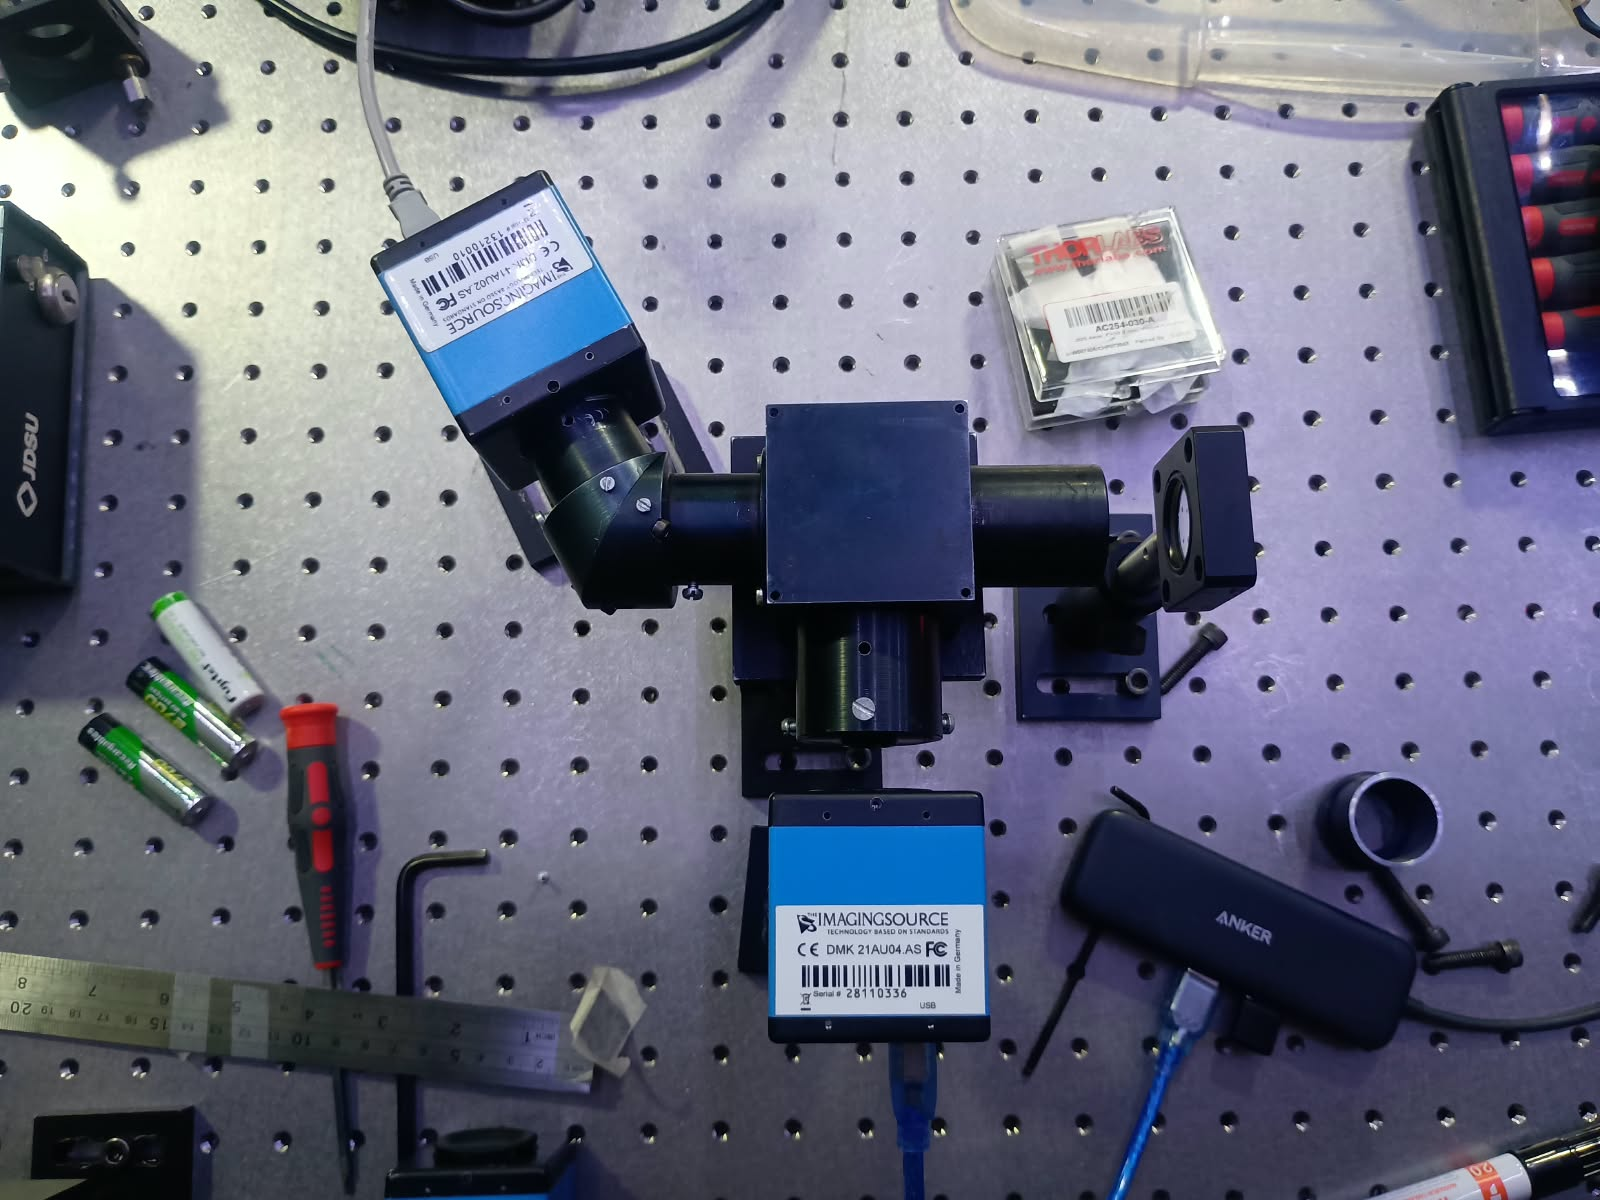
\includegraphics[width=0.85\linewidth]{montaje_besos.jpeg}
\caption{Setup: BESOS head (centre), spectrum camera DMK~41AU02.AS on the inclined port (top left), slit-viewer camera DMK~21AU04.AS (bottom) and the feeding lens mount (right).}
\label{fig:setup}
\end{figure}

For each source \NFrames{} frames were taken (gain 354--392, gamma 104, \SIrange{1}{150}{\milli\second} exposure, chosen to avoid saturation except for the flash). The reduction, implemented in a Python package, proceeds as follows: (i) median combination of the frames; (ii) tracing of a Kr line row by row and quadratic fit $x(y)$, used to shift every row so that the curved lines become vertical; (iii) extraction of the 1D spectrum averaging rows 450--550, the best-focus region; (iv) Gaussian fits, simultaneous for blended features; (v) Hartmann calibration~\eqref{eq:hartmann} with isolated Ar and Kr lines; (vi) computation of $P$, $R$ and the range, and comparison with \eqref{eq:prism}--\eqref{eq:range}.

\section{Results}
\label{sec:results}

\subsection{Line curvature and extraction}
Dispersion runs along $x$, blue to the left. The slit images are not straight but parabolic, with a sagitta of $\sim$\CurvSagitta~px between rows 250 and 800 and a mean tilt of \CurvTilt$^\circ$ in the extracted region. The quadratic trace fits the centroids with \CurvRMS~px rms and removes the curvature (Fig.~\ref{fig:curv}). The line width also changes along the slit (Fig.~\ref{fig:fwhmrow}): it is minimum, $\sim$3~px, in rows 450--550 and grows to 5--7~px towards the ends, so only that band was extracted.

\begin{figure}[htbp]
\centering
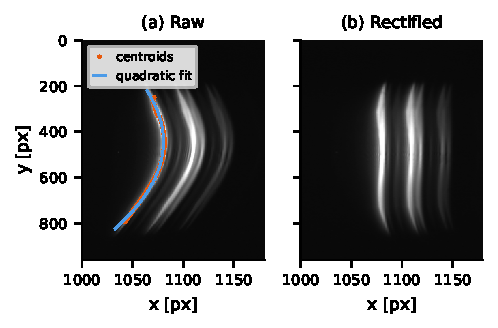
\includegraphics[width=\linewidth]{curvatura_lineas.pdf}
\caption{Kr lines around 760--830~nm. (a) Raw frame with the centroids of the traced line and the quadratic fit. (b) Same region after rectification.}
\label{fig:curv}
\end{figure}

\begin{figure}[htbp]
\centering
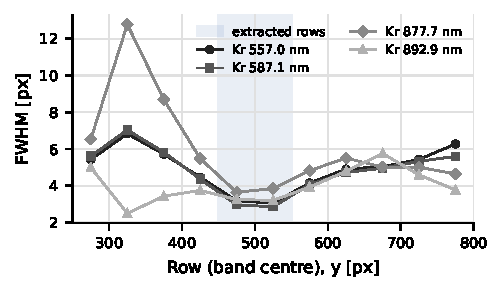
\includegraphics[width=\linewidth]{fwhm_vs_fila.pdf}
\caption{FWHM of four isolated Kr lines measured in 50-row bands along the slit. The shaded band marks the extracted rows.}
\label{fig:fwhmrow}
\end{figure}

\subsection{Line identification and wavelength calibration}
The lamps used were the following: the white lamp is krypton (weak lines at 557.0 and 587.1~nm, strong ones at 758--830~nm) and the rose one is argon (696.5, 706.7, 763.5, 811.5, 912.3, 965.8~nm). Fig.~\ref{fig:gauss} shows the profiles and Gaussian fits of all sources. The LEDs are 20--27~nm wide, far broader than the atomic lines, so they are used only as an independent check. Of the \NFeatures{} fitted lamp features, \CalN{} are isolated lines; the rest are unresolved blends and were not used.

\begin{figure*}[htbp]
\centering
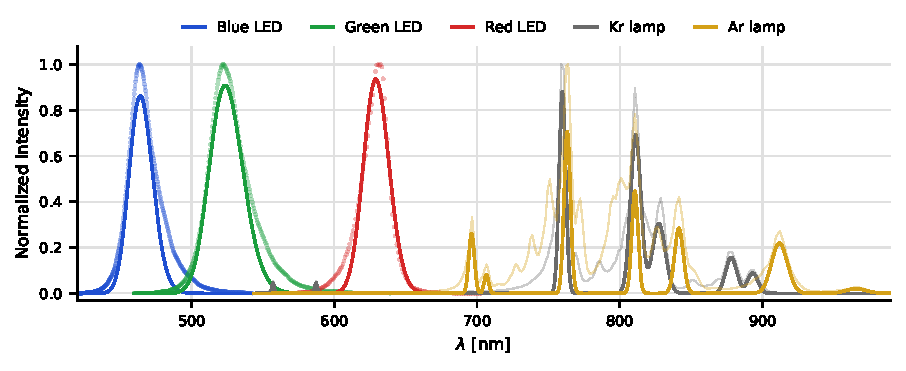
\includegraphics[width=\textwidth]{gaussianas_leds_lamparas.pdf}
\caption{Spectral profiles (faint) and Gaussian fits (solid) of the three LEDs and of the Kr and Ar lamps, normalized to the peak of each source and plotted with the final calibration.}
\label{fig:gauss}
\end{figure*}

The Hartmann fit to the \CalN{} isolated lines gives $\lambda_0=\HartLamZero$~nm, $C=$~\HartC~nm\,px and $x_0=\HartXzero$~px, with residuals of \CalRMS~nm rms (Fig.~\ref{fig:cal}, Table~\ref{tab:lines}). Applied to the LEDs, which were not in the fit, it places them at \LEDBlue, \LEDGreen{} and \LEDRed~nm (Table~\ref{tab:leds}), consistent with typical blue, green and red LEDs. This also checks the blue end, where the calibration is an extrapolation.

\begin{figure}[htbp]
\centering
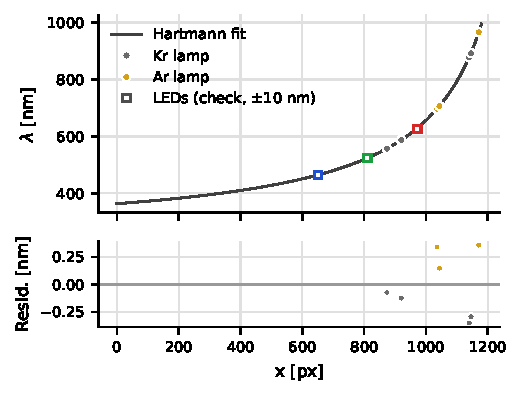
\includegraphics[width=\linewidth]{calibracion.pdf}
\caption{Hartmann calibration with the isolated Kr and Ar lines (top) and its residuals (bottom). The LEDs (squares, nominal $\lambda\pm10$~nm) are not part of the fit.}
\label{fig:cal}
\end{figure}

\begin{table}[htbp]
\caption{Isolated lines: laboratory wavelength [nm], centroid, calibration residual [nm], FWHM, reciprocal dispersion, resolution element and resolving power.}
\label{tab:lines}
\centering
\scriptsize
\setlength{\tabcolsep}{3pt}
\begin{tabular}{@{}lrrrrrrr@{}}
\toprule
Lamp & $\lambda_{\rm lab}$ & $x$ [px] & Resid. & FWHM [px] & $P$ [nm/px] & $\Delta\lambda$ [nm] & $R$ \\
\midrule
Kr & 557.0 & 873.7 & $-$0.07 & 3.1 & 0.59 & 1.9$\pm$0.1 & 301 \\
Kr & 587.1 & 920.0 & $-$0.13 & 2.9 & 0.71 & 2.1$\pm$0.1 & 283 \\
Ar & 696.5 & 1035.7 & +0.34 & 3.7 & 1.24 & 4.6$\pm$0.3 & 153 \\
Ar & 706.7 & 1043.8 & +0.15 & 2.8 & 1.30 & 3.7$\pm$0.8 & 191 \\
Kr & 877.7 & 1139.7 & $-$0.35 & 3.8 & 2.45 & 9.2$\pm$0.4 & 95 \\
Kr & 892.9 & 1145.8 & $-$0.29 & 3.2 & 2.57 & 8.3$\pm$0.7 & 107 \\
Ar & 965.8 & 1171.0 & +0.36 & 5.3 & 3.18 & 16.8$\pm$0.8 & 58 \\
\bottomrule
\end{tabular}

\end{table}

\begin{table}[htbp]
\caption{LED positions from the calibration (fit error only).}
\label{tab:leds}
\centering
\footnotesize
\begin{tabular}{@{}lccc@{}}
\toprule
Source & $\lambda_{\rm nom}$ & $\lambda_{\rm meas}$ [nm] & FWHM [nm] \\
\midrule
Blue LED & 465 & 464.2$\pm$0.6 & 19.4 \\
Green LED & 525 & 523.6$\pm$0.4 & 27.4 \\
Red LED & 625 & 629.2$\pm$0.2 & 21.1 \\
\bottomrule
\end{tabular}

\end{table}

\subsection{Dispersion}
The measured reciprocal dispersion is the derivative of the calibration, $P=|C|/(x-x_0)^2$ (Fig.~\ref{fig:disp}). It grows from \DispMeasFiveH~nm/px at 500~nm to \DispMeasSixH~nm/px at 600~nm and \DispMeasEightH~nm/px at 800~nm. Its shape follows the SF18 prism (the ratio to the model varies only \DispRatioSpread\% over 440--970~nm), but its value is \DispRatio{} times the design one: the spectrum is more compressed than expected, maybe due to the camera being at 27~mm instead of 40~mm.

\begin{figure}[htbp]
\centering
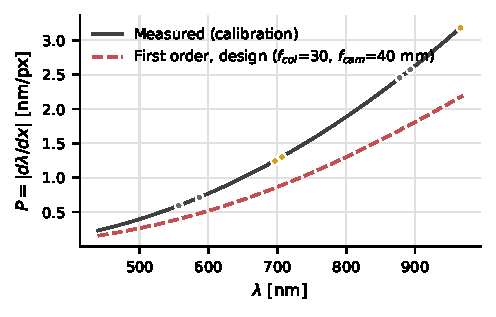
\includegraphics[width=\linewidth]{dispersion.pdf}
\caption{Measured reciprocal dispersion (derivative of the calibration; dots at the calibration lines) and first-order design value.}
\label{fig:disp}
\end{figure}

\subsection{Resolution}
The isolated Kr lines have a median FWHM of \FWHMKr~px and the Ar lines \FWHMAr~px. The resolution element grows from about 2~nm at 557--587~nm to 17~nm at 966~nm, and the resolving power falls from $R\approx\RMax$ to $R\approx\RMin$ (Table~\ref{tab:lines}, Fig.~\ref{fig:res}). The measured values are above the design curve at all wavelengths covered by Kr.

\begin{figure}[htbp]
\centering
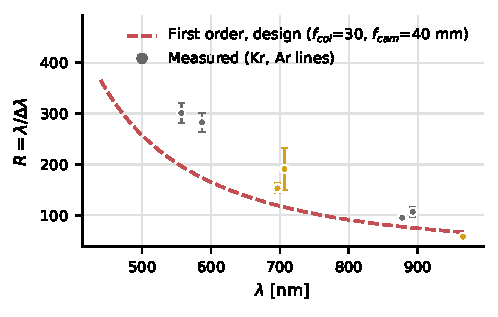
\includegraphics[width=\linewidth]{resolucion.pdf}
\caption{Measured resolving power (Kr grey, Ar yellow) and first-order design value for a \SI{25}{\micro\meter} slit.}
\label{fig:res}
\end{figure}

\subsection{Spectral range}
\label{sec:range}
The flash spectrum (Fig.~\ref{fig:flash}) shows the pump LED peak near 450~nm, the dip near 480~nm and the broad phosphor band. With a \RangeThr\% threshold the range is \RangeMin--\RangeMax~nm. \FlashSat\% of the flash pixels are saturated, which flattens 520--610~nm. The calibration places the blue edge of the detector ($x=0$) at \RangeDetMin~nm, and the Ar line at \RangeLastLine~nm was detected at the red end, so the instrument covers at least \RangeDetMin--\RangeLastLine~nm and the flash range is set by the source.

\begin{figure}[htbp]
\centering
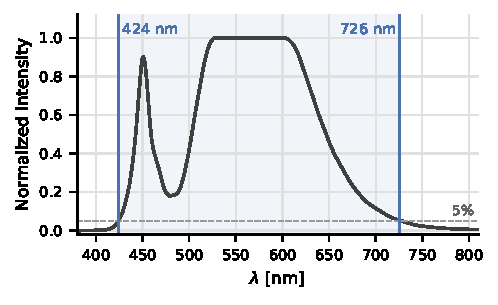
\includegraphics[width=\linewidth]{flash_rango.pdf}
\caption{Phone flash spectrum and range defined at \RangeThr\% of the peak.}
\label{fig:flash}
\end{figure}

\begin{table}[htbp]
\caption{Summary: first-order design vs.\ measured values.}
\label{tab:summary}
\centering
\footnotesize
\begin{tabular}{@{}lcc@{}}
\toprule
Parameter & Design & Measured \\
\midrule
$P$ at 500 nm [nm/px] & 0.26 & 0.39 \\
$P$ at 600 nm [nm/px] & 0.52 & 0.77 \\
$P$ at 800 nm [nm/px] & 1.30 & 1.88 \\
Slit image FWHM [px] & 7.2 & 3.2 \\
$\Delta\lambda$ at 557 nm [nm] & 2.8 & 1.9 \\
$R$ at 557 nm & 197 & 301 \\
$R$ at 878 nm & 77 & 95 \\
Range [nm] & 416--$>$1000$^a$ & 424--726$^b$ \\
\bottomrule
\end{tabular}
\\[2pt]
\parbox{0.95\linewidth}{\scriptsize $^a$Detector limit with 550~nm centred. $^b$Flash, limited by the source; detector covers at least \RangeDetMin--\RangeLastLine~nm.}
\end{table}

\section{Discussion}
\label{sec:disc}

\emph{Dispersion and line width.} The reciprocal dispersion was found to be \DispRatio{} times the design value, and the lines (\FWHMKr~px) are narrower than the expected slit image (\SlitImgPx~px). Both effects can be explained by a prism rotated away from minimum deviation: at $\theta_1\approx\ThetaOff^\circ$ the anamorphic factor $r=\AnamOff$ reproduces the measured line width and accounts for a factor \DispRatioOff{} in $P$. The remaining $\sim$20\% is attributed to the real focal length of the camera doublet and the detector position, which were not measured.

\emph{Resolution.} $R$ lies above the design curve because the narrower lines more than compensate the lower dispersion. The instrument is slit limited ($R_{dif}$ is ten times larger) and the $\sim$3~px FWHM satisfies Nyquist sampling. The Ar values are the least reliable, due to blends and a less uniform illumination of the slit.

\emph{Range.} The flash range is limited by the source; the instrument covers at least \RangeDetMin--\RangeLastLine~nm. In the near infrared $P>2$~nm/px (700--970~nm span only \NPxNIR~px), so the useful range is the visible.

\emph{Error sources.} The blue calibration is an extrapolation (no lamp lines below 557~nm) checked only with LEDs of unknown wavelength, and the lamps were identified by their line pattern. The 8-bit format, the missing darks and the saturated flash affect the profiles more than the centroids.

\section{Conclusions}
\label{sec:concl}

The BESOS prism spectrograph was assembled and characterized with LEDs, Kr and Ar lamps and a phone flash. A Hartmann calibration on \CalN{} isolated lines reaches \CalRMS~nm rms and is confirmed independently by the three LEDs. The reciprocal dispersion is strongly non-linear, from \DispMeasFiveH~nm/px at 500~nm to \DispMeasEightH~nm/px at 800~nm. It has the shape expected for SF18 but is \DispRatio{} times the design value. The resolving power is slit limited, from $R\approx\RMax$ at 557~nm to $R\approx100$ at 880--890~nm, above the design expectation because the lines are narrower than the nominal slit image. The range measured with the flash is \RangeMin--\RangeMax~nm, limited by the source, while the instrument covers at least \RangeDetMin--\RangeLastLine~nm.

\begin{thebibliography}{9}
\bibitem{guide}
L. Vanzi, \emph{Astronomical Instrumentation Lab IEE3873 -- Construction of a small low resolution spectrometer for the visible}, course guidelines and \emph{Introduction to Low Resolution Spectrograph}, AIUC, Pontificia Universidad Cat\'olica de Chile.

\bibitem{besos}
CAOS -- Club of Amateurs in Optical Spectroscopy, \emph{BESOS: a prism spectrograph}. \url{https://spectroscopy.wordpress.com/2011/04/10/besos-a-prism-spectrograph/}

\bibitem{hartmann}
J. Hartmann, ``A simple interpolation formula for the prismatic spectrum,'' \emph{Astrophys. J.}, vol.~8, p.~218, 1898.

\bibitem{schott}
SCHOTT AG, optical glass data sheet, SF18 ($n_d=1.72151$, $V_d=29.25$).

\end{thebibliography}

\end{document}
